\documentclass[journal,12pt,twocolumn]{IEEEtran}
%
\usepackage{setspace}
\usepackage{gensymb}
\usepackage{siunitx}
\usepackage{tkz-euclide}
\usepackage{textcomp}
\usepackage{standalone}
%\doublespacing
\singlespacing
\usetikzlibrary{calc}
%\usepackage{graphicx}
%\usepackage{amssymb}
%\usepackage{relsize}
\usepackage[cmex10]{amsmath}
%\usepackage{amsthm}
%\interdisplaylinepenalty=2500
%\savesymbol{iint}
%\usepackage{txfonts}
%\restoresymbol{TXF}{iint}
%\usepackage{wasysym}
\usepackage{amsthm}
%\usepackage{iithtlc}
\usepackage{mathrsfs}
\usepackage{txfonts}
\usepackage{stfloats}
\usepackage{bm}
\usepackage{cite}
\usepackage{cases}
\usepackage{subfig}
%\usepackage{xtab}
\usepackage{longtable}
\usepackage{multirow}
%\usepackage{algorithm}
%\usepackage{algpseudocode}
\usepackage{enumitem}
\usepackage{mathtools}
\usepackage{steinmetz}
\usepackage{tikz}
\usepackage{circuitikz}
\usepackage{verbatim}
\usepackage{tfrupee}
\usepackage[breaklinks=true]{hyperref}
%\usepackage{stmaryrd}
\usepackage{tkz-euclide} % loads  TikZ and tkz-base
%\usetkzobj{all}
\usetikzlibrary{calc,math}
\usepackage{listings}
    \usepackage{color}                                            %%
    \usepackage{array}                                            %%
    \usepackage{longtable}                                        %%
    \usepackage{calc}                                             %%
    \usepackage{multirow}                                         %%
    \usepackage{hhline}                                           %%
    \usepackage{ifthen}                                           %%
  %optionally (for landscape tables embedded in another document): %%
    \usepackage{lscape}    
\usepackage{multicol}
\usepackage{chngcntr}
%\usepackage{enumerate}

%\usepackage{wasysym}
%\newcounter{MYtempeqncnt}
\DeclareMathOperator*{\Res}{Res}
%\renewcommand{\baselinestretch}{2}
\renewcommand\thesection{\arabic{section}}
\renewcommand\thesubsection{\thesection.\arabic{subsection}}
\renewcommand\thesubsubsection{\thesubsection.\arabic{subsubsection}}

\renewcommand\thesectiondis{\arabic{section}}
\renewcommand\thesubsectiondis{\thesectiondis.\arabic{subsection}}
\renewcommand\thesubsubsectiondis{\thesubsectiondis.\arabic{subsubsection}}

% correct bad hyphenation here
\hyphenation{op-tical net-works semi-conduc-tor}
\def\inputGnumericTable{}                                 %%

\lstset{
%language=C,
frame=single,
breaklines=true,
columns=fullflexible
}
%\lstset{
%language=tex,
%frame=single,
%breaklines=true
%}

\begin{document}
%


\newtheorem{theorem}{Theorem}[section]
\newtheorem{problem}{Problem}
\newtheorem{proposition}{Proposition}[section]
\newtheorem{lemma}{Lemma}[section]
\newtheorem{corollary}[theorem]{Corollary}
\newtheorem{example}{Example}[section]
\newtheorem{definition}[problem]{Definition}
%\newtheorem{thm}{Theorem}[section] 
%\newtheorem{defn}[thm]{Definition}
%\newtheorem{algorithm}{Algorithm}[section]
%\newtheorem{cor}{Corollary}
\newcommand{\BEQA}{\begin{eqnarray}}
\newcommand{\EEQA}{\end{eqnarray}}
\newcommand{\define}{\stackrel{\triangle}{=}}
\bibliographystyle{IEEEtran}
%\bibliographystyle{ieeetr}
\providecommand{\mbf}{\mathbf}
\providecommand{\pr}[1]{\ensuremath{\Pr\left(#1\right)}}
\providecommand{\qfunc}[1]{\ensuremath{Q\left(#1\right)}}
\providecommand{\sbrak}[1]{\ensuremath{{}\left[#1\right]}}
\providecommand{\lsbrak}[1]{\ensuremath{{}\left[#1\right.}}
\providecommand{\rsbrak}[1]{\ensuremath{{}\left.#1\right]}}
\providecommand{\brak}[1]{\ensuremath{\left(#1\right)}}
\providecommand{\lbrak}[1]{\ensuremath{\left(#1\right.}}
\providecommand{\rbrak}[1]{\ensuremath{\left.#1\right)}}
\providecommand{\cbrak}[1]{\ensuremath{\left\{#1\right\}}}
\providecommand{\lcbrak}[1]{\ensuremath{\left\{#1\right.}}
\providecommand{\rcbrak}[1]{\ensuremath{\left.#1\right\}}}
\theoremstyle{remark}
\newtheorem{rem}{Remark}
\newcommand{\sgn}{\mathop{\mathrm{sgn}}}
\providecommand{\abs}[1]{\left\vert#1\right\vert}
\providecommand{\res}[1]{\Res\displaylimits_{#1}} 
\providecommand{\norm}[1]{\left\lVert#1\right\rVert}
%\providecommand{\norm}[1]{\lVert#1\rVert}
\providecommand{\mtx}[1]{\mathbf{#1}}
\providecommand{\mean}[1]{E\left[ #1 \right]}
\providecommand{\fourier}{\overset{\mathcal{F}}{ \rightleftharpoons}}
%\providecommand{\hilbert}{\overset{\mathcal{H}}{ \rightleftharpoons}}
\providecommand{\system}{\overset{\mathcal{H}}{ \longleftrightarrow}}
	%\newcommand{\solution}[2]{\textbf{Solution:}{#1}}
\newcommand{\solution}{\noindent \textbf{Solution: }}
\newcommand{\cosec}{\,\text{cosec}\,}
\providecommand{\dec}[2]{\ensuremath{\overset{#1}{\underset{#2}{\gtrless}}}}
\newcommand{\myvec}[1]{\ensuremath{\begin{pmatrix}#1\end{pmatrix}}}
\newcommand{\mydet}[1]{\ensuremath{\begin{vmatrix}#1\end{vmatrix}}}
%\numberwithin{equation}{section}
\numberwithin{equation}{subsection}
%\numberwithin{problem}{section}
%\numberwithin{definition}{section}
\makeatletter
\@addtoreset{figure}{problem}
\makeatother
\let\StandardTheFigure\thefigure
\let\vec\mathbf
%\renewcommand{\thefigure}{\theproblem.\arabic{figure}}
\renewcommand{\thefigure}{\theproblem}
%\setlist[enumerate,1]{before=\renewcommand\theequation{\theenumi.\arabic{equation}}
%\counterwithin{equation}{enumi}
%\renewcommand{\theequation}{\arabic{subsection}.\arabic{equation}}
\def\putbox#1#2#3{\makebox[0in][l]{\makebox[#1][l]{}\raisebox{\baselineskip}[0in][0in]{\raisebox{#2}[0in][0in]{#3}}}}
     \def\rightbox#1{\makebox[0in][r]{#1}}
     \def\centbox#1{\makebox[0in]{#1}}
     \def\topbox#1{\raisebox{-\baselineskip}[0in][0in]{#1}}
     \def\midbox#1{\raisebox{-0.5\baselineskip}[0in][0in]{#1}}
\vspace{3cm}
\title{Assignment 5}
\author{Neha Rani}
\maketitle
\newpage
%\tableofcontents
\bigskip
\renewcommand{\thefigure}{\theenumi}
\renewcommand{\thetable}{\theenumi}
\begin{abstract}
This document explains the the concept of finding the angle between the two straight lines from given second degree equation 
\end{abstract}
Download all latex-tikz codes from 
\begin{lstlisting}
https://github.com/neharani289/ee14014/tree/master/Assignment5
\end{lstlisting}
\section{Problem}
Prove that the equation $12x^2+7xy-10y^2+13x+45y-35=0$ represents two straight lines and find the angle between them 
\subsection{Pair of staraight lines}
The general second order equation is given by ,
\begin{align}
    ax^2+2bxy+cy^2+2dx+2ey+f&=0\label{eq1}
    \intertext{the above equation \eqref{eq1} can be expressed as}
    \vec{x}^T\vec{V}\vec{x}+2\vec{u}^T\vec{x}+f&=0\label{eq3}
    \intertext{where}
    \vec{V}=\vec{V}^T&=\myvec{a & b \\ b & c}\label{eq4}\\
    \vec{u}&=\myvec{d \\ e}\label{eq5}
    \end{align}
the above equation \eqref{eq1} represents a pair of straight lines if
\begin{align}
    \begin{array}{|cc|}
\vec{V} & \vec{u}\\\vec{u}^T & f
\end{array}&=0\label{eq6}
\end{align}
\section{Solution}
Given,
\begin{align}
    12x^2+7xy-10y^2+13x+45y-35&=0 \label{eqgiven}
\end{align}
The above equation can be expressed as
\begin{align}
        \vec{x}^{T}\vec{Vx} + 2\vec{u}^{T}\vec{x} + f=0   \label{eq:solutions/eq2}
\end{align}
where
\begin{align}
	\vec{V}=\vec{V}^T &= \myvec{12 & \frac{7}{2} \\ \frac{7}{2} & -10} \\
	\vec{u} &= \myvec{\frac{13}{2} \\ \frac{45}{2}} \\
	 f=-35
\end{align}	
	(\ref{eq:solutions/eq2}) represents a pair of straight lines if
\begin{align}
	&\mydet{\vec{V} & \vec{u} \\ \vec{u}^T & f} = 0     \label{eq:solutions/eq5} \\
	\mydet{\vec{V} & \vec{u} \\ \vec{u}^T & f} 
		&= \mydet{12 & \frac{7}{2}  & \frac{13}{2} \\ 
	        \frac{7}{2} & -10 & \frac{45}{2}     \\
	       \frac{13}{2} & \frac{45}{2} & -35 }  \\
	       		\nonumber \\
	\implies \ 12\mydet{-10 & \frac{45}{2} \\ \frac{45}{2} & -35} 
		& -\frac{7}{2}\mydet{\frac{7}{2} & \frac{45}{2} \\ \frac{13}{2} & -35} 
		+\frac{13}{2}\mydet{\frac{7}{2} & -10 \\ \frac{13}{2} & \frac{45}{2}} = 0 \label{eq:solutions/eq10}
\end{align}
The lines intercept if
\begin{align}
        \mydet{\vec{V}} < 0 \\
 	\mydet{\vec{V}}=-\frac{529}{4} < 0 \label{eq:solutions/eq11}
\end{align}
\renewcommand{\thefigure}{1}
From (\ref{eq:solutions/eq10}) and (\ref{eq:solutions/eq11}) it can be concluded that the given equation represents a pair of intersecting lines.



Let $(\alpha,\beta)$ be their point of intersection, then
\begin{equation}\label{eq6}
	\myvec{ a & b\\ b & c}\myvec{\alpha \\ \beta} = \myvec{-d \\ -e}
\end{equation}
Under \textit{Affine transformation},
\begin{align}
	\vec{x} &= \vec{M}\vec{y} + c\\
	\myvec{x \\ y} &= \myvec{1 & 0 \\ 0 & 1} \myvec{X \\ Y} + \myvec{\alpha \\ \beta}\\
	\label{eq7}\myvec{x \\ y} &= \myvec{X+\alpha \\ Y+\beta}
\end{align}
 under transformation \eqref{eq7} will become,
\begin{equation}\label{eq8}
	aX^2 + 2bXY + cY^2 = 0
\end{equation}
\begin{equation}\label{eq9}
	\myvec{X & Y} \myvec{a & b \\ b & c} \myvec{X \\ Y} = 0
\end{equation}
%\begin{equation}\label{eq10}
%	\vec{X}^T\vec{V}\vec{X} = 0
%\end{equation}
\begin{equation}\label{eq11}
	\myvec{X & Y} \myvec{u_1 & v_1 \\ u_2 & v_2} \myvec{\lambda_1 & 0\\ 0 & \lambda_2} \myvec{u_1 & u_2 \\ v_1 & v_2} \myvec{X \\ Y} = 0
\end{equation}
\begin{equation}
	\myvec{X^\prime & Y^\prime}  \myvec{\lambda_1 & 0\\ 0 & \lambda_2} \myvec{X^\prime \\ Y^\prime} = 0
\end{equation}
\begin{equation}\label{eq12}
	\text{where } X^\prime = Xu_1 + Yu_2 \text{ and } Y^\prime = Xv_1 + Yv_2
\end{equation}
\begin{equation}\label{eq13}
	\implies \lambda_1 (X^\prime)^2 + \lambda_2 (Y^\prime)^2 = 0
\end{equation}
\eqref{eq13} is called \textit{Spectral decomposition} of matrix
\begin{align}
	\implies X^\prime &= \pm \sqrt{-\frac{\lambda_2}{\lambda_1}}Y^\prime\\	
	u_1X + u_2Y &= \pm \sqrt{-\frac{\lambda_2}{\lambda_1}}(v_1X + v_2Y)\\
	\label{eq14}u_1(x-\alpha) + u_2(y-\beta) &= \pm \sqrt{-\frac{\lambda_2}{\lambda_1}}(v_1(x-\alpha) + v_2(y-\beta))
\end{align}
Substituting in \eqref{eq6}
\begin{align}
	\label{eq16}\myvec{ 12 & \frac{7}{2}\\\frac{7}{2} & -10}\myvec{\alpha \\ \beta} = \myvec{\frac{-13}{2} \\ -\frac{45}{2}} \\
	\label{eq17}\implies \myvec{\alpha \\ \beta} = \myvec{-1 \\ 2}
\end{align}
\begin{equation}
	\text{From \textit{Spectral theorem, }}\vec{V} = \vec{P}\vec{D}\vec{P}^T
\end{equation}
\begin{align}
	\label{eq18}\vec{V} &= \myvec{ 12 & \frac{7}{2}\\ \frac{7}{2} & -10}\\
	\label{eq19}\vec{P} &= \myvec{\frac{-\sqrt{533} - 22}{2} & \frac{-22 + \sqrt{533}}{2}\\ 1 & 1}\\
	\label{eq20}\vec{D} &= \myvec{1 + \frac{\sqrt{533}}{2} & 0\\ 0 & 1 - \frac{\sqrt{533}}{2}}
\end{align}
Substituting \eqref{eq17}, \eqref{eq19} and \eqref{eq20} in \eqref{eq14},
\begin{multline}\label{eq21}
	\frac{\sqrt{533}-22}{2}(x+1) + (y-2) \\= \pm \sqrt{-\frac{1 - \frac{\sqrt{533}}{2}}{1 + \frac{\sqrt{533}}{2}}}\left(\frac{-22 -\sqrt{533}}{2}(x+1) + (y-2)\right)
\end{multline}
Simplifying \eqref{eq21},
\begin{align}
	\label{eq22}3x -2y + 7 = 0 \text{ and } 4x + 5y -5 = 0\\
	\implies (3x - 2y + 7)(4x + 5y - 5) = 0
\end{align}
Thus the equation of lines are
\begin{align}
	\myvec{4 & 5}\vec{x} = 5 \\
	\myvec{3 & -2}\vec{x} = -7 
\end{align}
\begin{figure}[h]
    \centering
    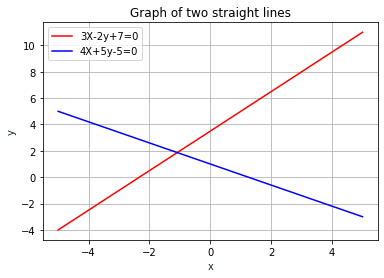
\includegraphics[width=\columnwidth]{Figure.png}
    \caption{Pair of straight lines}
    \label{Fig :1}
\end{figure}
\section{Angle between the straight lines}
The angle between the lines can be expressed in terms of normal vectors 
\begin{align}
	\vec{n_1}=\myvec{4\\5} , \quad \vec{n_2}=\myvec{3\\-2}
\end{align}
as
\begin{align}
	\cos\theta=\frac{\vec{n_1}^T\vec{n_2}}{\norm{\vec{n_1}}\norm{\vec{n_2}}} \\
				\nonumber \\
	\implies \quad \theta=\cos^{-1}({\frac{2}{\sqrt{533}}}) = \tan^{-1}(\frac{23}{2})
\end{align}
\end{document}
